% Created 2018-11-08 Thu 14:47
% Intended LaTeX compiler: pdflatex
\documentclass[11pt]{article}
\usepackage[utf8]{inputenc}
\usepackage[T1]{fontenc}
\usepackage{graphicx}
\usepackage{grffile}
\usepackage{longtable}
\usepackage{wrapfig}
\usepackage{rotating}
\usepackage[normalem]{ulem}
\usepackage{amsmath}
\usepackage{textcomp}
\usepackage{amssymb}
\usepackage{capt-of}
\usepackage{hyperref}
\usepackage{color}
\usepackage{minted}
\usepackage[margin=2cm]{geometry}
\author{John Harwell}
\date{\today}
\title{}
\begin{document}

\begin{center}
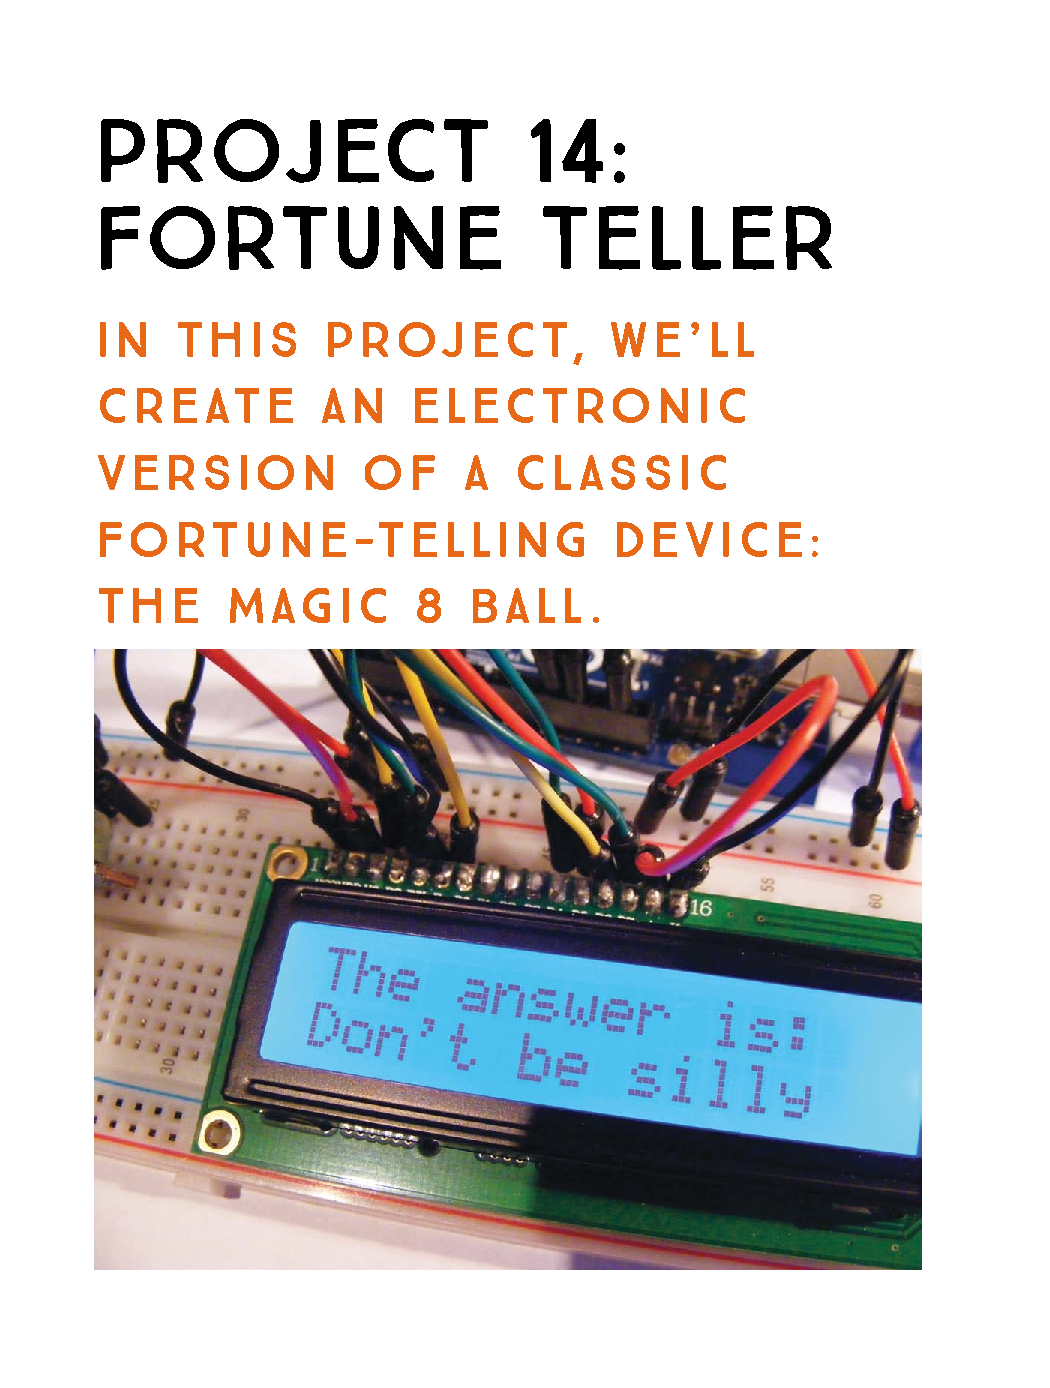
\includegraphics[width=.9\linewidth]{./exp4-magic-8ball-1.pdf}
\end{center}

\begin{center}
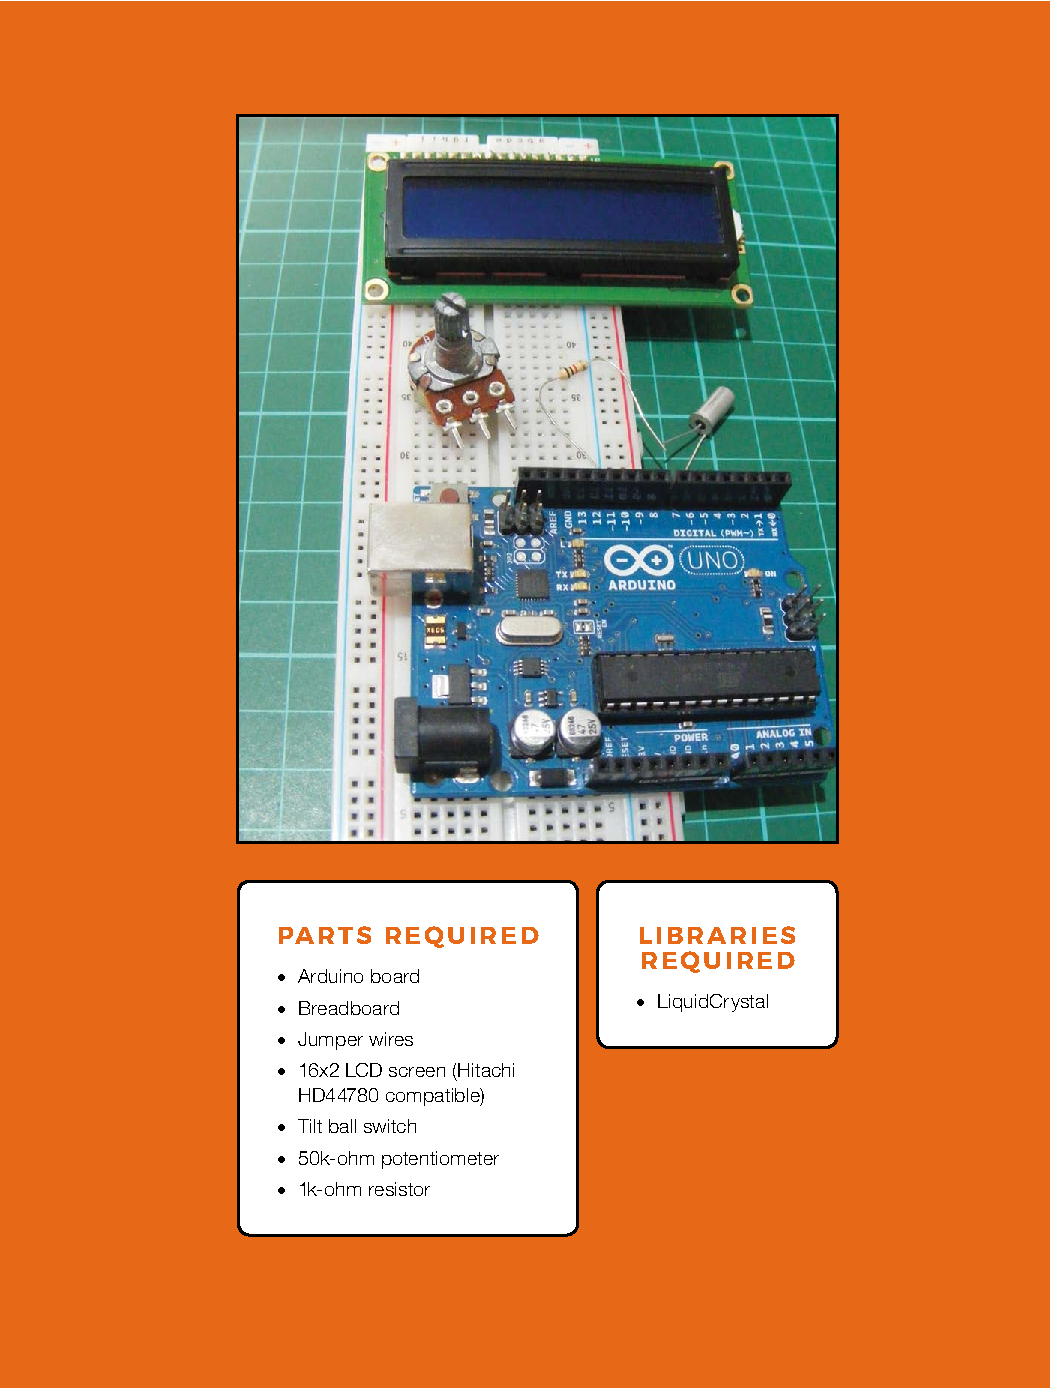
\includegraphics[width=.9\linewidth]{./exp4-magic-8ball-2.pdf}
\end{center}

\section{Setup}
\label{sec:org85ada87}

First you will need to download, unzip, and install the Arduino Integrated Development Environment (IDE) from
\url{https://www.arduino.cc/en/Main/Donate} (does not need admin privileges).

\section{How it works}
\label{sec:org0e1724c}

The Magic 8 Ball, a novelty toy created in the 1950s, is made of a hollow sphere in which a 20-sided die floated in
alcohol. When you ask the ball a question and shake it, one side of the die floats up and displays your answer in the
ball’s window. For this project, you'll use a random number generator (a computer version of rolling a die) that will
generate a number between 0 and 8 to simulate shaking the ball. In this project you will ask a question, and then press
the pushbutton on the circuit to get your answer.

The potentiometer is a variable valued resistor that controls how much electricity will flow to the LCD screen. More
electricity = brighter LCD, less electricity = dimmer LCD.

\texttt{QUESTION}

How does an LCD screen work? How does a potentiometer work, and when might they be useful? (hint: think of visual and
audio related devices)

\section{Building The Circuit}
\label{sec:org9f69d75}

The schematics for the circuits you will be building is below. The first schematic is for the LCD screen part, and the
second is for the pushbutton. You should substitute the pushbutton circuit where the tilt switch is in the first
schematic.

\begin{center}
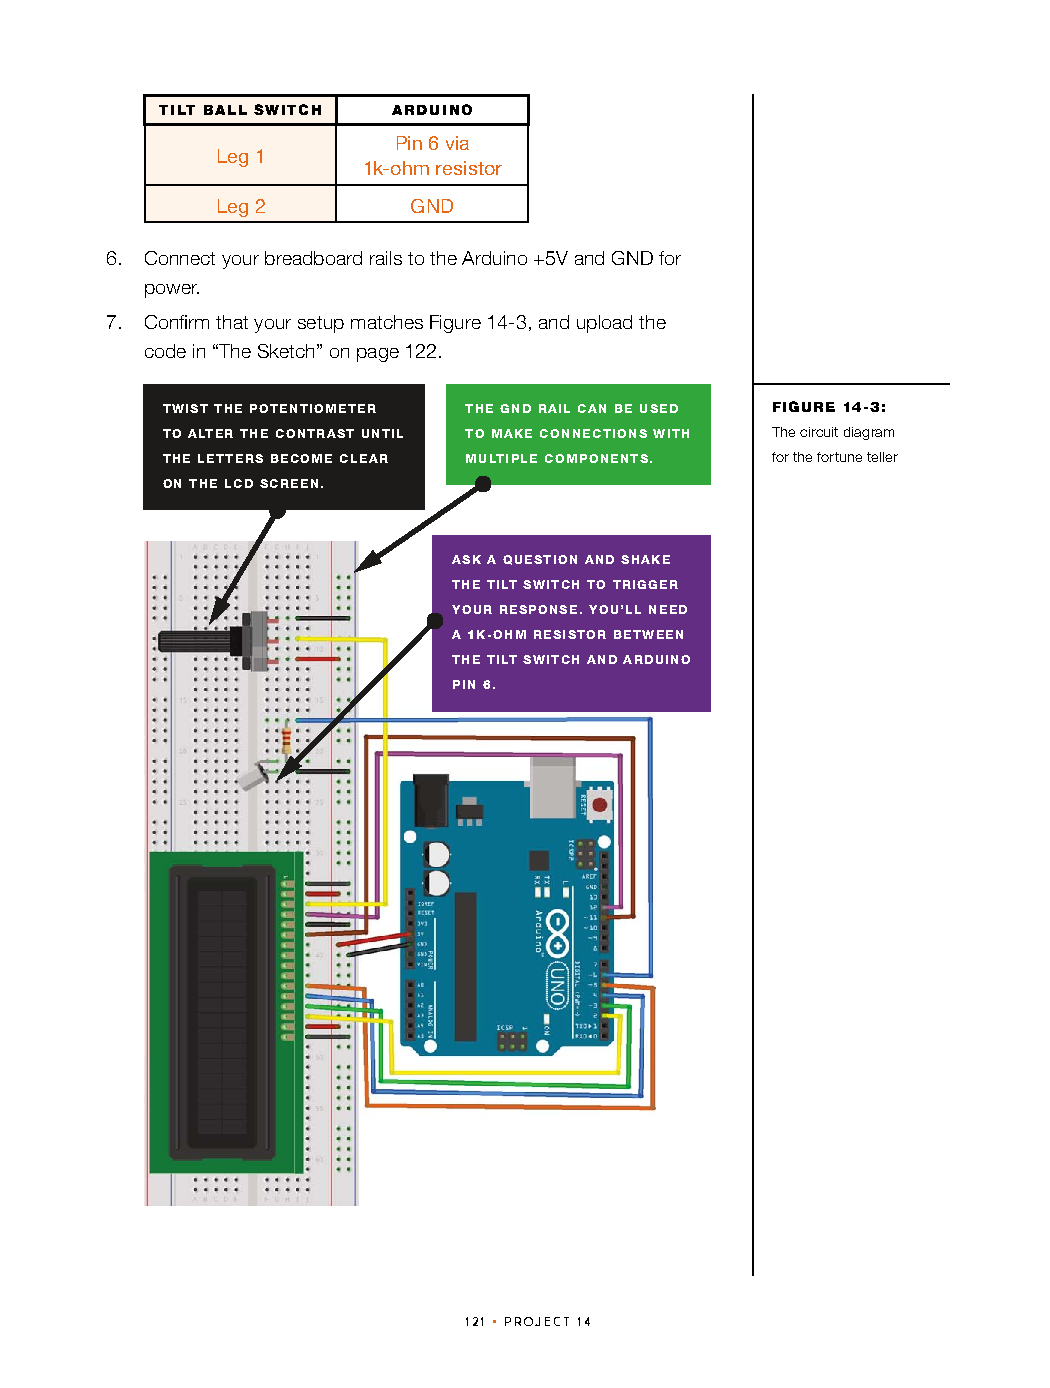
\includegraphics[width=.9\linewidth]{./exp4-magic-8ball-5.pdf}
\end{center}

\begin{center}
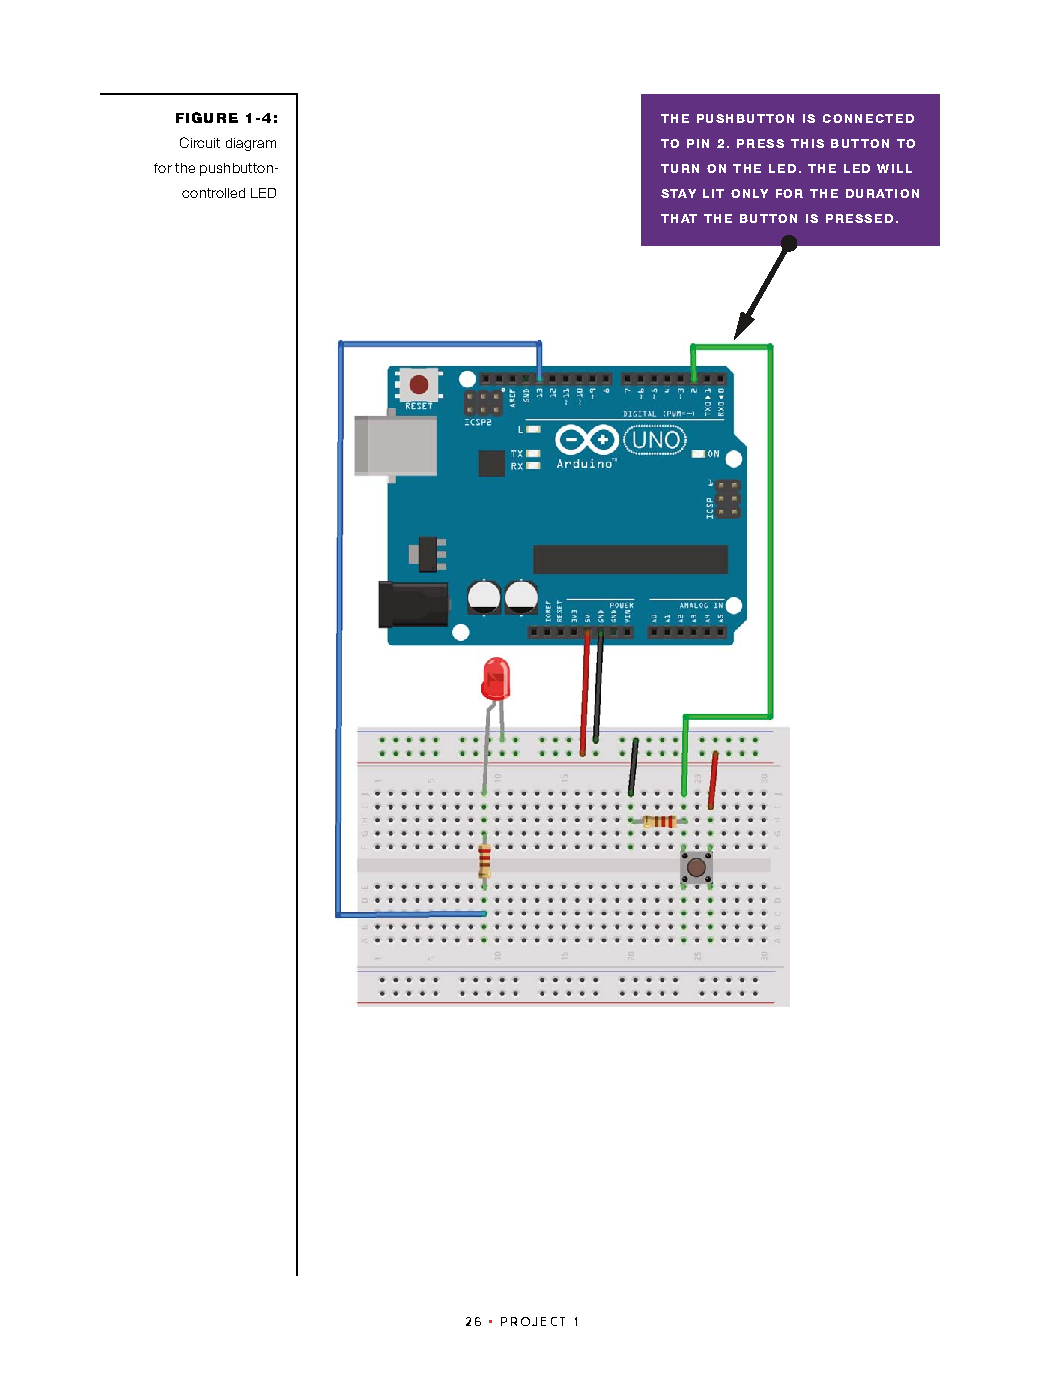
\includegraphics[width=.9\linewidth]{./exp4-magic-8ball-6.pdf}
\end{center}


\section{Programming the Arduino}
\label{sec:org654036c}

The base code for programming the Arduino is provided. Using the Arduino IDE, open the \texttt{.ino} file.

\texttt{PAUSE}

The IDE allows you to do 4 things: edit the code, verify the code is correct (i.e. does not contain syntax
errors), upload the code to the Arduino, and view the diagnostic output of things as they run on the Arduino.

Uploading to the Arduino is easy! Just click the Upload arrow in the IDE.

\section{The fortune teller code}
\label{sec:org4ee1087}

The fortune teller comes with a stock set of responses, you may want to change them to be something more to your
liking. You can modify what is between the quotes in the \texttt{lcd.print()} lines of the code. \texttt{lcd.print()} is a \emph{function},
meaning that it is a helper that you can ask to do something for you. In this case, you are asking it to tell the LCD
screen to print something specific for you.

The main part of the code is the \texttt{switch()} statement, which controls what the fortune teller's response will be. Each
time a new random number is generated (i.e. the computerized die is rolled), the resulting number is put into one of the
8 "boxes" of the switch statement. The switch statement acts as a set of boxes at a candy store: each type of candy that
comes it for an employee to stock has to be put in its correct box, and the contents of the boxes can't be mixed, or the
customers will be unhappy. The \texttt{switch()} statement does the same thing in the code!

\section{Extending The Code}
\label{sec:org5e8d97d}

Once you have the fortune teller working to your liking try the following:

\begin{itemize}
\item Increasing the number of fortunes from the original 8 to 10 (for example).
\item Change the code so that you have to HOLD the pushbutton while asking your question, and then release it to get the
answer.
\end{itemize}
\end{document}
